%%%%%%%%%%%%%%%%%%%%%%%%%%%%%%%%%%%%%%%%%%%%%%%%%%%%%%%%%%%%%%%%%%%%%%%%%%%%%%%%
%2345678901234567890123456789012345678901234567890123456789012345678901234567890
%        1         2         3         4         5         6         7         8
% THESIS CHAPTER


\chapter{Control Framework}
\label{chap:control}
\ifpdf
    \graphicspath{{ControlFramework/Figures/PNG/}{ControlFramework/Figures/PDF/}{ControlFramework/Figures/}}
\else
    \graphicspath{{ControlFramework/Figures/EPS/}{ControlFramework/Figures/}}
\fi

\section*{Introduction}
In this section, the implemented control framework is presented, along with the necessary mathematical details. The architecture is constituted by two parts:
\begin{itemize}
	\item The Mission Manager, which job is to supervise the execution of the overall mission. In this specific case, it is only a support for the subsequent part. It creates the \textit{action}, that are a lists of control objectives that the Kinematic Control Layer must satisfy during the mission phases. 
	\item The Kinematic Control Layer (KCL) focus on provide the system velocities (i.e. vehicle and joint velocities), given the list of control objectives from the Mission Manager.
\end{itemize}
This thesis focuses mostly on the Kinematic Control Layer. Discussions about how to implement a more complete Mission Manager (which acts not only as a support for the KCL, but, for example, it deals also with the \textit{planning} of the mission phases) go out the scope of this work.\\

The framework is build from the one used in \cite{IntroMaris2}, \cite{tesiWander}, and \cite{IntroRecent}. The sections \ref{sec:definitions}, \ref{sec:controlObjectives}, \ref{sec:tpik}, \ref{sec:armVehScheme}, and \ref{sec:coopScheme} derive from these works and in the following pages their main aspects are recalled.

\section{Definitions}
\label{sec:definitions}
In this section, the necessary definitions are presented. We will consider the general case of a floating manipulator, made up of an $l$-DOF arm attached to a 6-DOF vehicle.\\

\noindent Let us define:
\begin{itemize}
	\item The system configuration vector $ \boldsymbol{c} \in \mathbb{R}^{n}$ of the robot: ~
	$\boldsymbol{c} \triangleq 
		\begin{bmatrix}
			{\boldsymbol{q}} \\ \boldsymbol{\eta}
		\end{bmatrix}$,\\
	where $\boldsymbol{q} \in \mathbb{R}^{l}$ is the l-DOF arm configuration vector and  $\boldsymbol{\eta} \in \mathbb{R}^6$ is the vehicle \emph{generalized coordinate position vector}.\\
	The first three components of $\boldsymbol{\eta}$ form the position vector $\boldsymbol{\eta}_1 \triangleq \begin{bmatrix}x \\ y \\ z\end{bmatrix}$, with components in the inertial frame $\langle w \rangle$.\\
	The last three components of $\boldsymbol{\eta}$ forms the orientation vector $\boldsymbol{\eta}_2 \triangleq \begin{bmatrix}\phi \\ \theta \\ \psi\end{bmatrix}$ expressed in terms of the three angles roll, pitch, yaw (applied in the yaw-pitch-roll sequence \cite{fossenAnglesSeq}). The singularity given by this Euler sequence that arise when $ \theta = \pi/2$ is handled by a specific control objective, the \textit{horizontal attitude} (section \ref{sec:taskList}). As the name suggests, this objective assures the vehicle to stay away from the cited singularity.\\
	From the given definition, it results that $ n = l+6 $
	
	\item The system velocity vector $\dot{\boldsymbol{y}} \in \mathbb{R}^n$ of the robot: ~
	$\dot{\boldsymbol{y}} \triangleq 
	\begin{bmatrix}\dot{\boldsymbol{q}} \\ \boldsymbol{v}\end{bmatrix}$,\\
	where $\dot{\boldsymbol{q}} \in \mathbb{R}^{l}$ are the arm joint velocities and $\boldsymbol{v} \in \mathbb{R}^{6}$ is the vehicle velocity vector.\\
	The first three components of $\boldsymbol{v}$ form the linear velocities $\boldsymbol{v}_1 \triangleq \begin{bmatrix}\dot{x} \\ \dot{y} \\ \dot{z}\end{bmatrix}$ and the last three form the angular velocities $\boldsymbol{v}_2 \triangleq \begin{bmatrix}p \\ q \\ r\end{bmatrix}$, both with components in the vehicle frame $\langle v \rangle$. \\
	The vehicle is considered fully actuated, so the vector $\dot{\boldsymbol{y}}$ coincides with the control vector that is the output of the kinematic layer.
\end{itemize}
	
\section{Control Objectives}
\label{sec:controlObjectives}
Let us consider what the robot has to achieve. An \textit{objective} is a job that the robot must accomplish during the mission. Different objectives can be requested at the same time, for example we want the joints to stay away from their physical limits and the robot to maintain an horizontal attitude, while the end-effector is reaching a desired pose. \\
In the following, specific discussions about these objectives are made.
\subsection{Control Objectives classification}
\label{sec:coClass}
Control objectives can be classified depending on their importance (i.e. \textit{priority}) in the context of the mission. In fact, some of them can be more important than others. For example, usually we want to avoid an obstacle if this one is in the trajectory given by the reaching goal objective. So, we want \textit{before} to avoid the obstacle and \textit{then} to continue towards the goal. In general, the idea is that the more important objectives have to been satisfied first, and then, \textit{if possible}, also the less important ones. 
A general classification based on the \textit{priority} is given here (from the more important class to the less important one):
\begin{itemize}
	\item \textit{Physical Constraints} objectives. This class includes the interactions with the environment (e.g. not pushing against a rigid surface, imposing a cooperative tool velocity when two robots are carrying together the tool).
	\item \textit{System Safety} objectives. Usually (but not always), the safety is more important than the accomplishment of the Mission. As the name suggest, in this class there are objectives which aim to not damage anything (robot or objects), anyone (humans) and, in general, to not make the whole mission fail. Examples can be staying away from joint mechanical limits, or avoiding an obstacle.
	\item \textit{Prerequisite} objectives. This class is for objectives needed to accomplish the actual mission. An example for a grasping Mission could be focusing the camera on the object to be grasped.
	\item \textit{Mission} objectives, the actual objective that define the mission, like reaching an end-effector position.
	\item \textit{Optimization} objectives. This class is to choose, among all the possible solutions (if multiple ones exist) the best one. For example, this category can be used to improve the energy consumption.
\end{itemize}
The classes of \textit{priority} of these objectives are only a general classification. Depending on the application, objectives can have a different ordering.

\subsection{Equality and Inequality Control Objectives}
\label{sec:eqIneqObj}
Difference between equality and inequality control objectives is another important classification. We consider a variable  $ \boldsymbol{x}(\boldsymbol{c}) \in \mathbb{R}^m $, dependent on the robot configuration vector $ \boldsymbol{c}$, with $ m $ \textit{dimension} of the control objective. \\
The control objective can be of two types:
\begin{itemize}
	\item \textit{Equality control objective}, the requirement, for $t \to \infty$, that \\ \mbox{$\boldsymbol{x}(\boldsymbol{c}) = \boldsymbol{x}_0$}.
	
	\item \textit{Inequality control objective}, the requirement, for $t \to \infty$, that \\ \mbox{$\boldsymbol{x}(\boldsymbol{c}) < \boldsymbol{x}_{max}$ ~ or ~ $\boldsymbol{x}(\boldsymbol{c}) > \boldsymbol{x}_{min}$ ~or ~$ \boldsymbol{x}_{min} < \boldsymbol{x}(\boldsymbol{c}) < \boldsymbol{x}_{max}$}.
\end{itemize}
Please note that here symbols $= , < , >$ refers to element-by-element comparison of the vectors.\\
To make the notations lighter, from now on the dependency of the variable $\boldsymbol{x}(\boldsymbol{c})$ on the configuration vector $\boldsymbol{c}$ will be omitted.\\
The importance of the subdivision between \textit{equality} and \textit{inequality} will be clarified later.

\subsection{Reactive and non Reactive Control Task}
\label{sec:reactNonReact}
Mathematically speaking, the aim of a control objective is to drive the variable $\boldsymbol{x}(\boldsymbol{c})$ toward a point $ \boldsymbol{x}^* $ where the requisite (introduced in the previous section \ref{sec:eqIneqObj}) is satisfied.
For this scope, each control objective has always associated a \textit{feedback reference rate} (in this thesis also denotes as \textit{reference velocity}).\\
An example of \textit{feedback reference rate} is:
\begin{equation}
	\label{feedbackRate}
	\boldsymbol{\dot{{\bar{x}}}} (\boldsymbol{x}) \triangleq \gamma (\boldsymbol{x}^* - \boldsymbol{x}),\quad \gamma > 0
\end{equation}
That is a simple proportional law, where $\gamma$ is a positive gain proportional to the desired convergence rate for the considered variable. From now on, the \textit{feedback reference rate} will have always this formulation.\\

To link the considered variable $ \boldsymbol{x}(\boldsymbol{c})$ to the system velocity vector $\dot{\boldsymbol{y}}$, the following relationship is used:
\begin{equation}
\label{eq:CartJacVel}
	\dot{\boldsymbol{x}} = \boldsymbol{J} \dot{\boldsymbol{y}}
\end{equation} 
that expresses how the system velocity vector $\dot{\boldsymbol{y}}$ influences the rate of change of the variable $\boldsymbol{x}$. $ \boldsymbol{J} \in \mathbb{R}^{m \times n}$ is the so-called \textit{task-induced Jacobian}.\\
The aim of having the actual $\dot{\boldsymbol{x}}$ as much as possible equal to the desired reference $\dot{\bar{\boldsymbol{x}}}$ is called a \textit{reactive control task}.\\

There are situations where a task has not an associated control objective. It happens when an external agent (e.g. an human operator with a console) provides directly the reference rate. So, there is no \textit{feedback reference rate} to calculate, because it is generated by the external agent. In the case of the human operator, it is this one that, seeing (in some way) how the system is behaving, adjust the command, making in its brain a sort of law like the one in formula \eqref{feedbackRate}.  When no control objective is present, we speak about \textit{non-reactive control task}.

%As an example, we take the objective is to drive the end-effector in a desired pose, with only the arm and considering a fixed vehicle. This problem is well know as \textit{inverse kinematic} problem; i.e. finding the joint velocities $\dot{\boldsymbol{q}} \in \mathbb{R}^l$ which bring the pose $\boldsymbol{x} \in \mathbb{R}^6$ in a specific one. In this case we have:
%\begin{equation}
%\dot{\boldsymbol{x}} = \begin{bmatrix}
%	\underset{3\times3}{\boldsymbol{J_{k,0}}} & \underset{3\times3}{\boldsymbol{0}} \\  \underset{3\times3}{\boldsymbol{0}} & \underset{3\times3}{^{w}\boldsymbol{R}_v}
%	\end{bmatrix}	
%	\dot{\boldsymbol{q}}	
%\end{equation}

\subsection{Inequality Control Objectives Activation and Deactivation}
\label{sec:activations}
During the execution of a mission, not always each inequality control objective is relevant. As an example, maintaining joints away from their mechanical limits is a safety objective which is needed only when the joints are actually near their limits. When a joint is sufficiently far away, there is no necessity to overconstrain the system imposing an additional velocity.\\
To deal with this, we speak about \textit{activation} and \textit{deactivation} of control objectives and of their relative control tasks.
Let us define the following \textit{activation function}:
\begin{equation}
	a(x) \in [0,1]
\end{equation}
as a continuous, sigmoidal, function, which assumes $0$ values within the validity region of the control objective. The validity region is intended as an interval where the objective is satisfied and it is far from not being satisfied any more (with satisfying we intend to accomplish the requirement explained in section \ref{sec:eqIneqObj}). At the margin of this region, a smooth transition from 0 to 1 is present, to gently activate/deactivate the control objective when necessary.\\
For example, considering a scalar ($ m = 1 $) inequality control objective with the requirement $x(\boldsymbol{c}) > x_{min}$ the \textit{activation function} can be defined as:
\begin{equation}
	\label{eq_activation_f}
	a(x) \triangleq
	\begin{cases}1,& x(\boldsymbol{c}) < x_{min}\\
	s(x),& x_{min} \leq x(\boldsymbol{c}) \leq x_{min} + \Delta\\
	0, & x(\boldsymbol{c}) > x_{min} + \Delta\\
	\end{cases}
\end{equation}    
where $s(x)$ is a smooth decreasing function joining the two extreme value $1$ and $0$, and $\Delta$ a value to create a zone where the inequality is satisfied but we want the objective to be activated a bit because we are near the margins. This is also important to prevent chattering problems that would occur if the objective was activated instantaneously.\\
Similar definitions of the activation function can be done for the other two kinds of inequality control objectives.\\

In general, for multidimensional control objectives ($m > 1$), the activation takes the form of a diagonal matrix:
\begin{equation}
\boldsymbol{A} \triangleq
	\begin{bmatrix}
	a_1 & & \\
	& \ddots & \\
	& & a_m	 
	\end{bmatrix}
\end{equation}
where the diagonal elements $a_i$ are activation functions defined similarly to the one in formula \eqref{eq_activation_f}.

Obviously, for the equality control tasks the activation function is a constant equal to $1$, because these tasks are always \enquote{active}. In the multidimensional case, the activation is an identity matrix.\\
Same reasoning can be done for the \textit{non-reactive} control tasks, being absent the variable $x(\boldsymbol{c})$, and being the reference velocities directly given.


\section{Task Priority Inverse Kinematics}
\label{sec:tpik}
In this section, the core of the control architecture is explained.\\
We describe an \textit{Action} $\mathcal{A}$ as a list of prioritized control objectives (with their associated tasks), each one positioned at a defined priority level $k$ (where lower $k$ means higher priority). With this notation, the following symbols are defined:
\begin{itemize}
	\item $\dot{\bar{\boldsymbol{x}}}_k \triangleq \begin{bmatrix}\dot{\bar{x}}_{1,k} & \cdots & \dot{\bar{x}}_{k_m,k}\end{bmatrix}^T$ is the vector of the reference velocities for the control task $k$, with a task dimension $k_m$.
	\item $\dot{\boldsymbol{x}}_k \triangleq \begin{bmatrix}\dot{x}_{1,k} & \cdots & \dot{x}_{k_m,k}\end{bmatrix}^T$ is the current rate of change of the task $k$.
	\item $\boldsymbol{J}_k$ is the Jacobian relationship which relates the current rate-of-change $\dot{\boldsymbol{x}}_k$ with the system velocity vector $\dot{\boldsymbol{y}}$ as in equation \eqref{eq:CartJacVel}.
	\item $\boldsymbol{A}_k \triangleq \textrm{diag}(a_{1,k},  \cdots,  a_{k_m,k})$ is the diagonal matrix composed by the activation functions described in section \ref{sec:activations}.
\end{itemize}
It is important to notice that, in the practice, different objectives can have the same priority. In this case, it is possible to simply stack the vectors and matrices to obtain a objective and a related task $k$ that includes both objectives. For simplicity, but without loss of generality, different objectives will be considered always at different priority levels.\\

The aim of the kinematic layer is to find a system velocity vector $\dot{\bar{\boldsymbol{y}}}$ that satisfies \textit{as much as possible} the requirements of each objective of the action $\mathcal{A}$. Given the presence of different objectives with different priorities, we have to satisfy first the higher priority ones, and then, \textit{if possible}, the lower priority ones. To do this, a sequence of nested minimization problems must be solved: 
\begin{equation}\label{eq:rminproblem}
S_k \triangleq \left\{ \arg \mathrm{R\textrm{-}}\min_{\dot{\bar{\boldsymbol{y}}} \in S_{k-1}} \left\| \boldsymbol{A}_k (\dot{\bar{\boldsymbol{x}}}_k - \boldsymbol{J}_k \dot{\bar{\boldsymbol{y}}}) \right\|^2 \right\},\, k = 1, 2, \ldots, N,
\end{equation}
where $S_0 \triangleq \mathbb{R}^n$, $\:S_{k-1}$ is the manifold of solutions of all the previous tasks in the hierarchy, and $N$ is the total number of priority levels. The notation $\mathrm{R\textrm{-}}\min$ is introduced in \cite{IntroMaris1}, and it indicates a series of regularization to avoid singularities.\\
This problem is the so called \textit{Task Priority Inverse Kinematics} (TPIK). To solve the formula  \eqref{eq:rminproblem}, the so called \textit{iCAT} (inequality Constraints And Task transitions) framework uses the following algorithm \ref{alg:icat}:
\begin{algorithm}[H]
	\caption{iCAT} \label{alg:icat}
	\begin{algorithmic} [1] {\large
		\STATE{$\boldsymbol{\rho}_{0} = \boldsymbol{0}$}
		\STATE{$\boldsymbol{Q}_{0} = \boldsymbol{I}$}
		\vspace{5px}
		\FOR{k=1 \TO N}
		\vspace{5px}
		\STATE{$\boldsymbol{W}_k =  \boldsymbol{J}_k \boldsymbol{Q}_{k-1} (\boldsymbol{J}_k \boldsymbol{Q}_{k-1})^{\#,\boldsymbol{A}_k,\boldsymbol{Q}_{k-1}}$}
				\vspace{5px}
		\STATE{$\boldsymbol{Q}_k = \boldsymbol{Q}_{k-1} (\boldsymbol{I} - (\boldsymbol{J}_k \boldsymbol{Q}_{k-1})^{\#,\boldsymbol{A}_k,\boldsymbol{I}} {\boldsymbol{J}_k \boldsymbol{Q}_{k-1}})$}
		\vspace{5px}
		\STATE{$\boldsymbol{\rho}_k = \boldsymbol{\rho}_{k-1} + \textrm{Sat}\left( \boldsymbol{Q}_{k-1} (\boldsymbol{J}_k \boldsymbol{Q}_{k-1})^{\#,\boldsymbol{A}_k,\boldsymbol{I}} \boldsymbol{W}_k \left(\dot{\bar{\boldsymbol{x}}}_k - \boldsymbol{J}_k \boldsymbol{\rho}_{k-1} \right) \right)$}
		\vspace{5px}
		\ENDFOR 
		\vspace{5px}
		\STATE{  $\dot{\bar{\boldsymbol{y}}} = \boldsymbol{\rho}_N$  }
	}
	\end{algorithmic}
\end{algorithm}

\noindent The special pseudo inverse operator $\boldsymbol{(\cdot)}^{\#,\boldsymbol{A},\boldsymbol{Q}}$ [\cite{IntroMaris1}] manages some invariance problems of \eqref{eq:rminproblem}; the function Sat($\cdot$) [\cite{antoSat}] controls the variable saturations. Details of the procedure can be found again in [\cite{IntroMaris1}].

\subsection{Notes on Conflicting Objectives}
From section \ref{sec:coClass}, it should be understood that lower priority tasks are not always satisfied. The problem with this arises when the main mission objective (e.g. reaching a point with the end effector), that is not at the higher priority, can't be never accomplished, thus failing the general mission. This can be the case when an obstacle is met: the robot may stuck in a point of \textit{local minima} (that is however better than crash into it). This means that the robot can't find a trajectory toward the goal and, \textit{at the same time}, avoids the obstacle. So, it remains still because avoiding the obstacle is an objective with more priority. This is a general problem of all reactive control methods. The solution must be found at the mission manager level, which should plan another trajectory (e.g. with intermediate way-points) and/or another sequence of Actions. This problem is not considered in this work. 



\section{Arm-Vehicle Coordination Scheme}
\label{sec:armVehScheme}
\begin{figure}[H]
	\begin{center}
		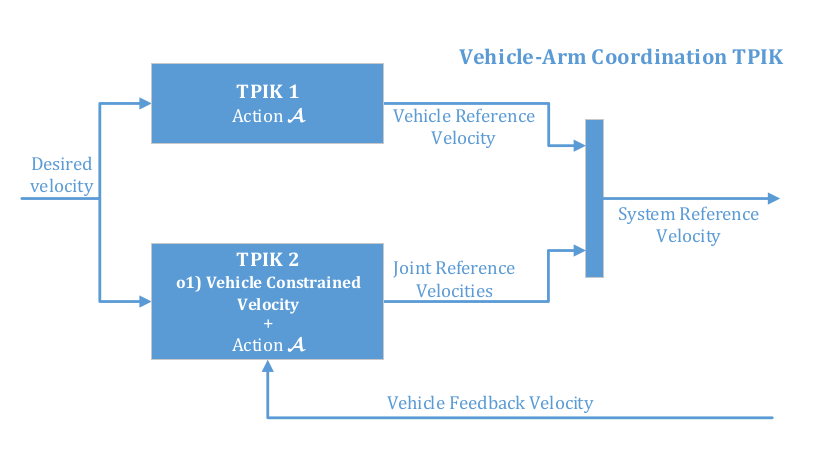
\includegraphics[width=0.90\columnwidth]{vehArmCoordScheme}
		\caption[Arm-Vehicle Coordination Scheme in the TPIK]{A scheme showing the two Task Priority Inverse Kinematics blocks for the arm-vehicle coordination}\label{fig:veharmcoord}
	\end{center}
\end{figure}
Inaccuracies in velocity tracking of the vehicle can have effects on the arm. 
A relevant problem arises when disturbances of the floating base, caused by thrusters and/or its large inertia, propagate and affect the end effector motions [\cite{IntroMaris2}].
To solve this, a kinematic decoupling of the arm and the base is done, implementing it within the task priority approach.\\
As in the previous sections, we consider an Action $\mathcal{A}$, that is a list of prioritized objectives to be satisfied.
The idea is to have two TPIK running in parallel as shown in figure \ref{fig:veharmcoord}:
\begin{itemize}
	\item \textbf{TPIK 1}. It considers the vehicle together with the arm as a whole full controllable system. From its output $\dot{\bar{\boldsymbol{y}}}$, only the vehicle velocity component are taken (discarding the arm ones).
	\item \textbf{TPIK 2}. It considers the vehicle as totally non controllable. So, a \textit{non-reactive} task (\ref{sec:reactNonReact}) is added at the top of the priority list $\mathcal{A}$ to \textit{constrain} the output vehicle velocity to the real one (measured in some way). The other objectives of $\mathcal{A}$ remain unchanged. From its output $\dot{\bar{\boldsymbol{y}}}$, only the arm part is taken.
\end{itemize}
At the end of the procedure, the two parts of $\dot{\bar{\boldsymbol{y}}}$ are put togheter to compose the final system reference velocity vector.\\
Thanks to the TPIK 2, the joint velocities are \textit{optimized}, in the sense that they follow \textit{at best} the objectives of the action $\mathcal{A}$ considering also the \textit{measured} vehicle velocity and its influence on the objectives.	

For real mobile manipulators, in general, a multi-rate control of arm and vehicle is used, which means that velocities for the arm and for the vehicle are given at different frequency. This is common because usually the arm can be controlled more precisely and its performance are better than the base. The coordination schema proposed here is suitable for such an implementation: the TPIK 2 can run at higher frequency, updating the commanded arm velocities more frequently than the vehicle ones.

\section{Cooperation Scheme}
\label{sec:coopScheme}
\begin{figure}[H]
	%\begin{center}
	\centerline{
		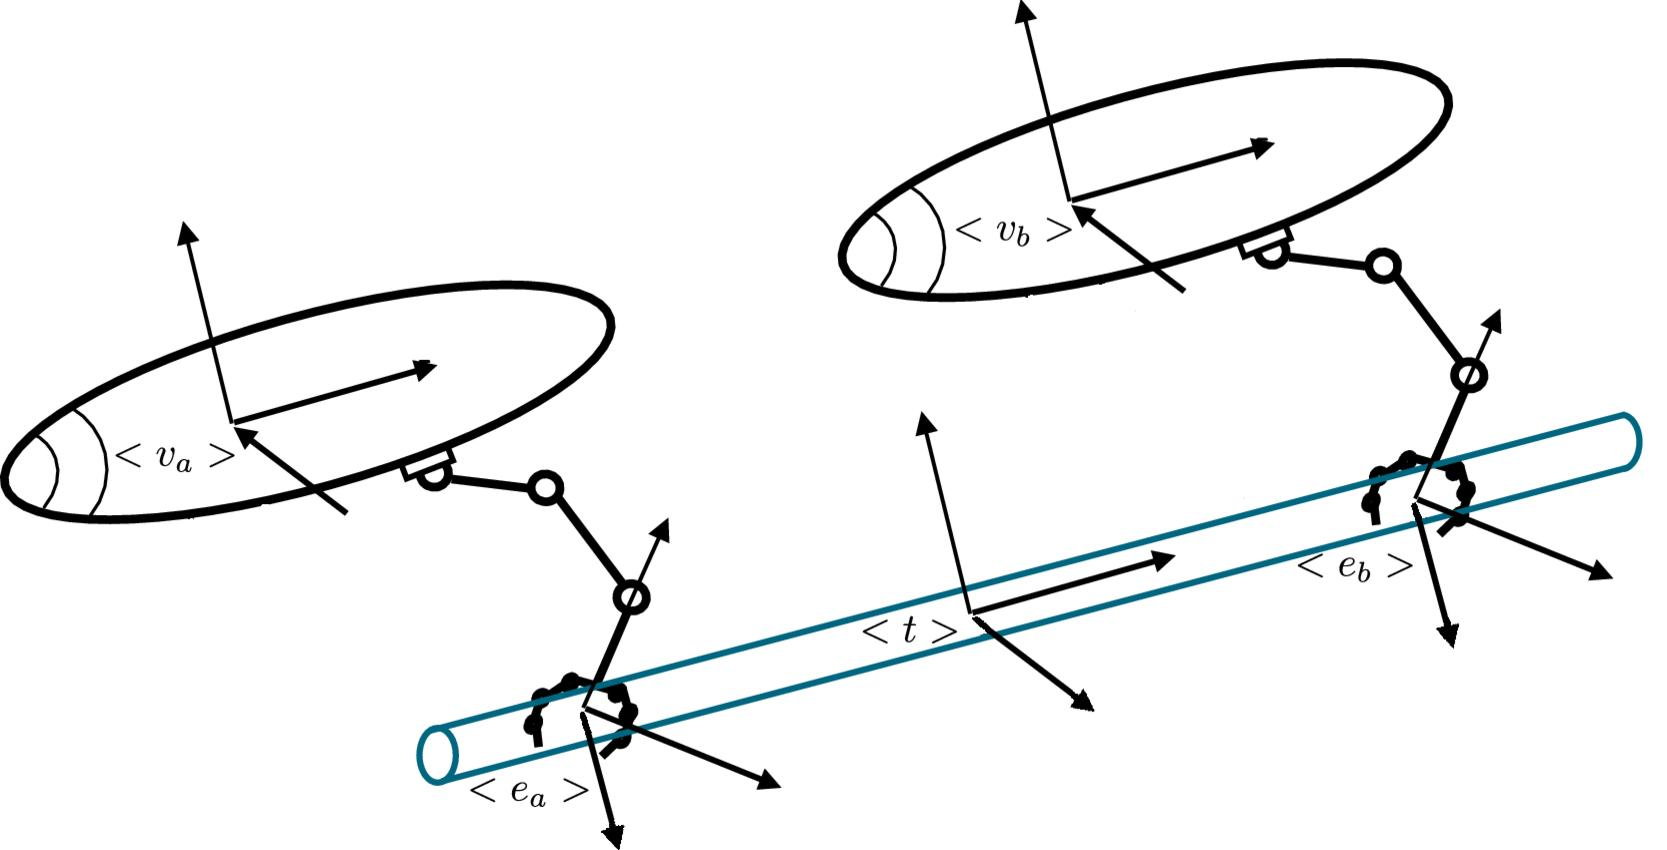
\includegraphics[width=0.8\columnwidth]{coopFrames.jpg}
	}
		\caption[Relevant frames for the cooperation scheme]{The frames of the two cooperative vehicles carrying a common object}\label{fig:coopFrames}
	%\end{center}
\end{figure}

In this section, the discussion about cooperation is explained. We limit the explanations to only two cooperative robotic systems, but, in general, more agents can be considered.\\

The \textit{cooperation} is used to carry a common tool with the two manipulators, without making it fall or break. This is done at kinematic level: the scheme provides suitable system velocities $\dot{\bar{\boldsymbol{y}}}_a$ and $\dot{\bar{\boldsymbol{y}}}_b$ for the two robots considering the constraint given by the carried common object. So, both system velocities $\dot{\bar{\boldsymbol{y}}}_a$ and $\dot{\bar{\boldsymbol{y}}}_b$ must cause same Cartesian velocity $\dot{{\boldsymbol{x}}}_t$ to the tool.\\
The coordination policy that will be presented takes care of the bandwidth restriction typical of underwater scenarios. Thus, it deals with the cooperation in a decentralized manner, limiting as much as possible the amount of data exchanged.\\
Furthermore, this scheme is different from the classical \textit{leader-follower} ones, because, as we will see, the \enquote{leadership} changes based on the difficulties in tracking the ideal tool velocity that one robot can meet.\\

It is assumed that the object is held firmly by both agents, so no sliding happens during the missions. The two robots agree on a shared fixed frame, so, their respective tool frames $\langle t_a \rangle$ and $\langle t_b \rangle$ and the object frame $\langle o \rangle$ are coincident: 
\begin{equation} 
\langle t \rangle \triangleq \langle t_a \rangle = \langle t_b \rangle = \langle o \rangle
\end{equation}
In figure \ref{fig:coopFrames} the main frames related to the cooperation are shown.\\

\noindent The firm grasp assumption imposes that:
\begin{equation}\label{eq:coopintro}
	\dot{\boldsymbol{x}}_t = \boldsymbol{J}_{t,a} \dot{\boldsymbol{y}}_a = \boldsymbol{J}_{t,b} \dot{\boldsymbol{y}}_b
\end{equation}
with $\dot{\boldsymbol{x}}_t$ the object velocity with component on $\langle t \rangle$; $\dot{\boldsymbol{y}}_a$, $\dot{\boldsymbol{y}}_b$ the system velocity vectors of agents $a$ and $b$ (introduced in section \ref{sec:definitions}); and $\boldsymbol{J}_{t,a}$, $\boldsymbol{J}_{t,b}$ the system Jacobians of agents $a$ and $b$ with respect to $\langle t \rangle$. These Jacobians tell how the tool velocity $\dot{\boldsymbol{x}}_t$ is affected by the system velocities $\dot{\boldsymbol{y}}_a$ and $\dot{\boldsymbol{y}}_b$. Due to the firm grasp assumption, the tool velocities caused by $\dot{\boldsymbol{y}}_a$ and $\dot{\boldsymbol{y}}_b$ must be equal.\\

\noindent Let us rewrite the second part of equation \eqref{eq:coopintro} as:
\begin{equation}\label{eq:coopintro2}
	\begin{gathered}
	\begin{bmatrix}
	\boldsymbol{J}_{t,a} & -\boldsymbol{J}_{t,b}
	\end{bmatrix}
	\begin{bmatrix}
	\dot{\boldsymbol{y}}_a \\ \dot{\boldsymbol{y}}_b
	\end{bmatrix}
	\triangleq \boldsymbol{G}\dot{\boldsymbol{y}}_{ab}=0 \quad \Longleftrightarrow \quad \dot{\boldsymbol{y}}_{ab} \in ker(\boldsymbol{G})
	\end{gathered}
\end{equation}
$ker(\boldsymbol{G})$ represents the subspace where $\dot{\boldsymbol{y}}_{ab}$ is constrained to lay for the firm grasp assumption.\\

We could consider the two manipulators as a unique system simply stacking correctly vectors and matrices. To transport cooperatively the tool, an additional \textit{physical constraint} objective would be added to the TPIK list, to ensure the control outputs a command $\dot{\bar{\boldsymbol{y}}}$ which satisfies the constraint \eqref{eq:coopintro2}. In practice, with this new objective, in the minimization problems of \eqref{eq:rminproblem} we would have $S_1 = ker(\boldsymbol{G})$.\\
The problem with following this way is that we are not considering that the two vehicles are separate entities. This idea would be feasible when the agent is a single robot with two arms. Instead, in this case, exchanging all the vectors and matrices between the robots during the TPIK procedure would not be possible, especially in an underwater situation. So, another method must be considered.\\

\noindent The equation \eqref{eq:coopintro} can be expressed in the Cartesian space as:
\begin{equation}
	\dot{\boldsymbol{x}}_t = \boldsymbol{J}_{t,a} \boldsymbol{J}^\#_{t,a} \dot{\boldsymbol{x}}_t =  \boldsymbol{J}_{t,b} \boldsymbol{J}^\#_{t,b} 
	\dot{\boldsymbol{x}}_t 
\end{equation}
\begin{equation}
\label{eq:constrainMatrixC}
	(\boldsymbol{J}_{t,a} \boldsymbol{J}^\#_{t,a} - \boldsymbol{J}_{t,b} \boldsymbol{J}^\#_{t,b}) 
	\dot{\boldsymbol{x}}_t \triangleq \boldsymbol{C} \dot{\boldsymbol{x}}_t = \boldsymbol{0}
\end{equation}
\begin{equation}
	\dot{\boldsymbol{x}}_t \in ker(\boldsymbol{C}) = Span(\boldsymbol{I} - \boldsymbol{C}^\#\boldsymbol{C})
\end{equation}
$\boldsymbol{C}$ is a particular matrix called \textit{Cartesian Constraint Matrix}. The kernel of $\boldsymbol{C}$ expresses the space of achievable object velocities at the current configurations of the two robots.\\

The idea of the scheme is to put a non-reactive task at the top of the hierarchy, to constrain the desired object velocity $\boldsymbol{\dot{\tilde{x}}}$ in this subspace. After this constraint, we are sure, at kinematic level, that both agents can follow this desired object velocity despite the possible different situations caused by the other objectives and by the different robots configurations.\\
\begin{figure}[H]
	\centering
	\centerline{
		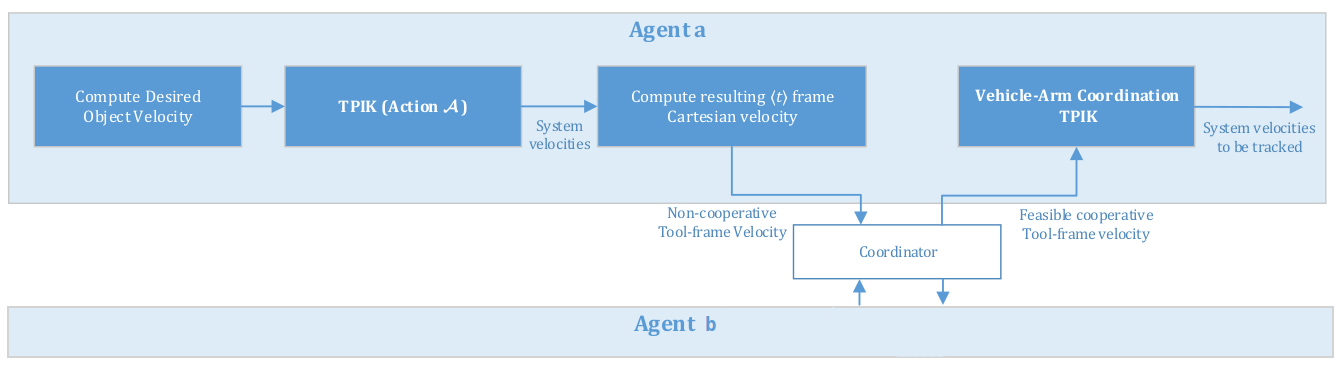
\includegraphics[width=1.22\columnwidth]{coopScheme2.png} }
	\caption[Cooperation Scheme in the TPIK]{The cooperation scheme with its different steps. The Agent b block is equal to the Agent a one.}
	\label{fig:coopScheme}
\end{figure}
\vspace{10px}
\noindent The scheme, sketched in figure \ref{fig:coopScheme} proceeds as follows:
\begin{itemize}
	\item In the first step, the two agents calculate system velocities (using the TPIK explained in  section \ref{sec:tpik}) as if they were alone. So, we have:
	\begin{equation}
		\dot{\boldsymbol{x}}_{t,a} = \boldsymbol{J}_{t,a} \dot{\boldsymbol{y}}_{a} , \qquad 
		\dot{\boldsymbol{x}}_{t,b} = \boldsymbol{J}_{t,a} \dot{\boldsymbol{y}}_{b}	
	\end{equation}
	where, in general, the two \textit{non cooperative} tool velocities are different:\\ \mbox{$\dot{\boldsymbol{x}}_{t,a} \neq \dot{\boldsymbol{x}}_{t,b}$.}
	
	\item The tool velocities are exchanged (i.e. they are sent to the coordinator) and a \textit{cooperative} tool velocity $\dot{\hat{\boldsymbol{x}}}_t$ is computed as:
	\begin{equation}\label{eq:weightsum}
		\dot{\hat{\boldsymbol{x}}}_t = \dfrac{1}{\mu_a + \mu_b} (\mu_a \dot{\boldsymbol{x}}_{t,a}  + \mu_b \dot{\boldsymbol{x}}_{t,b}), \qquad
		\mu_a , \mu_b > 0	
	\end{equation}
    \begin{equation}
		\begin{gathered}
			\mu_a = \mu_0 + \| \dot{\bar{\boldsymbol{x}}}_t - \dot{\boldsymbol{x}}_{t,a} \| \triangleq \mu_0 + \| \boldsymbol{e}_a \|, \\
			\mu_b = \mu_0 + \| \dot{\bar{\boldsymbol{x}}}_t - \dot{\boldsymbol{x}}_{t,b} \| \triangleq \mu_0 + \| \boldsymbol{e}_b \|, \\
			\mu_0 > 0
	    \end{gathered}
	\end{equation}
	where $\dot{\bar{\boldsymbol{x}}}_t$ is the ideal velocity that, if applied, would asymptotically take the tool to the desired goal.\\
	The \textit{cooperative} tool velocity $\dot{\hat{\boldsymbol{x}}}_t$  is a \textit{weighted} compromise between the two \textit{non cooperative} ones. The \textit{weights} $\mu_a, \mu_b$ give more freedom to the robot which meet the highest error $\boldsymbol{e}$. This error is a way to understand how much one robot is in difficult in tracking the \textit{ideal} tool velocity $\dot{\bar{\boldsymbol{x}}}_t$.
	
	\item The new \textit{cooperative} tool velocity $\dot{\hat{\boldsymbol{x}}}_t$ is not, in general, a \textit{feasible} velocity that both vehicle can provide to the tool. So, an additional passage is required:
	\begin{equation}
		\dot{\tilde{\boldsymbol{x}}}_t \triangleq \big( \boldsymbol{I} - \boldsymbol{C}^\# \boldsymbol{C} \big) \dot{\hat{\boldsymbol{x}}}_t
	\end{equation}
	with $\boldsymbol{C}$ defined in \eqref{eq:constrainMatrixC}.
	
	\item Each agent runs a new TPIK procedure, with a objective list identical to the first one, but with a \textit{non-reactive} control objective at the top to track the \textit{feasible cooperative} velocity $\dot{\tilde{\boldsymbol{x}}}_t$. The outputs of this procedure, $\dot{\hat{\boldsymbol{y}}}_a$ and $\dot{\hat{\boldsymbol{y}}}_b$ will be the final velocities which the kinematic layer provides.\\
	Moving the equality control objective to make the end effector reach the goal at the top of the hierarchy does not influence the safety tasks. This property is proven in \cite{tesiWander}.
\end{itemize}
\vspace{15px}
The method assumes that the Coordinator can calculate the ideal tool velocity $\dot{\bar{\boldsymbol{x}}}_t$, so it must know the transformation matrix between the goal frame $\langle g \rangle $ and the tool frame $ \langle t \rangle $.\\

It can be noticed how the only information that the agents must exchange are the 
\textit{non-cooperative} velocities $\dot{\boldsymbol{x}}_{t,a}$ and $\dot{\boldsymbol{x}}_{t,b}$, the matrices $\boldsymbol{J}_{t,a} \boldsymbol{J}^{\#}_{t,a}$ and $\boldsymbol{J}_{t,b} \boldsymbol{J}^{\#}_{t,b}$ (to build the Cartesian Constraint Matrix $\boldsymbol{C}$), and the feasible velocity $\dot{\tilde{\boldsymbol{x}}}_t$. Less data can be exchanged if we have Jacobians expressed analytically. In this case, instead of sharing the two $6 \times 6$ matrices, we can share only two configuration vectors $\boldsymbol{c}$ ($n \times 1$), and make the coordinator calculate the Jacobians from their analytical expressions.\\
Even less data can be shared if the \textit{coordinator} is a procedure that runs on a robot, and it is not on an external node. In this case, practically only half of the amount of data must be shared through water.